\section{Příklad 2}
% Jako parametr zadejte skupinu (A-H)
\druhyZadani{D}
\begin{figure}[H]
		\center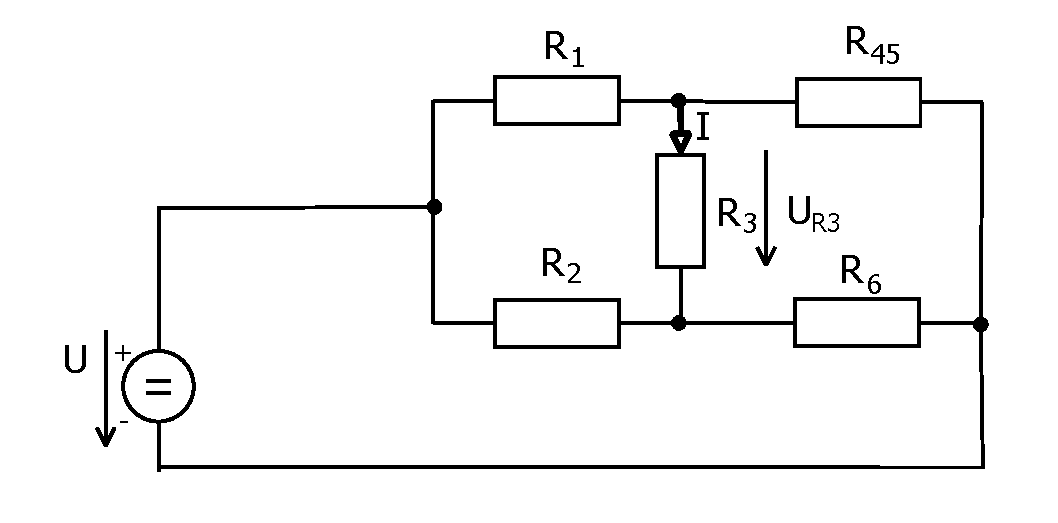
\includegraphics[width=0.6\linewidth]{obr/2_1.pdf}
		\caption{$R_4$ a $R_5$ si můžeme zapojit do série}
	\end{figure}
Spojíme si odpory ${R_4}$ a ${R_5}$
\begin{gather*}
R_{45} = R_4 + R_5 = 200 + 550 = 750\Omega \\
\end{gather*}


\begin{figure}[H]
		\center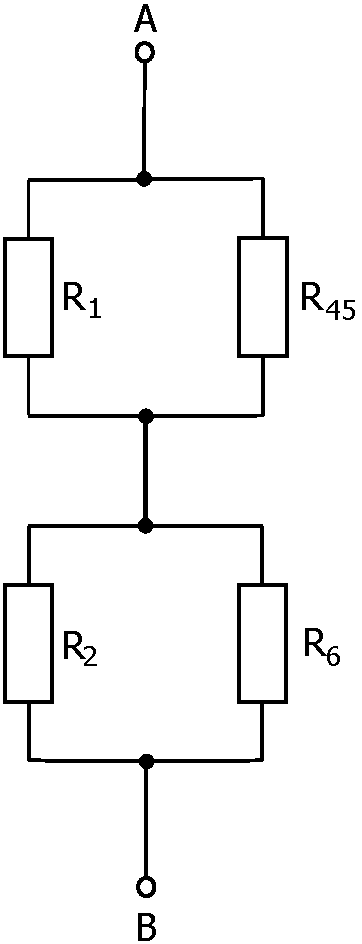
\includegraphics[width=0.25\linewidth]{obr/2_2.pdf}
		\caption{Obvod bez napěťového zdroje}
	\end{figure}
Postupným zjednodušením získáme odpor ${R_i}$:	
\begin{gather*}
R_I = \frac{R_{1}\cdot R_{45}}{R_{1} + R_{45}}+\frac{R_{2}\cdot R_{6}}{R_{2} + R_{6}} = \frac{200\cdot 750}{200 + 750}+\frac{200\cdot 400}{200 + 400}\doteq 291.22807 \Omega\\
\end{gather*}

\begin{figure}[H]
		\center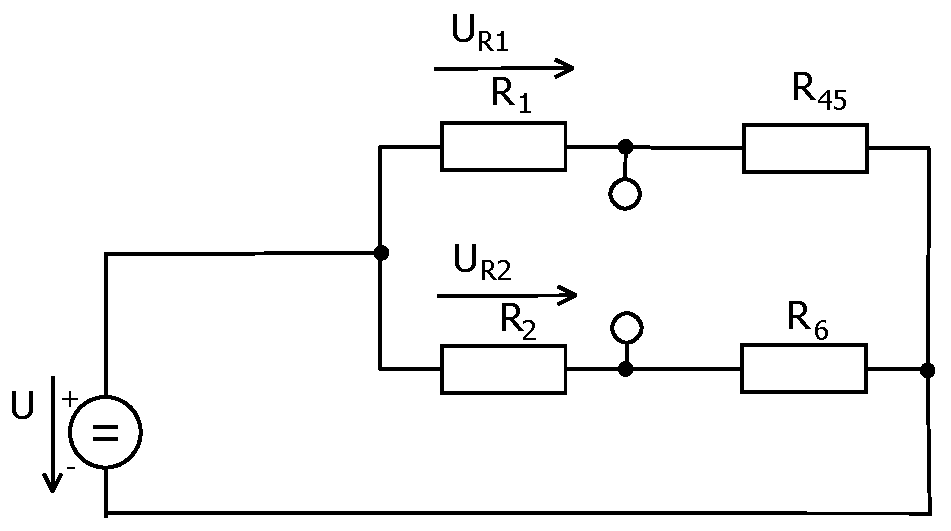
\includegraphics[width=0.6\linewidth]{obr/2_4.pdf}
		\caption{obvod bez ${R_3}$}
	\end{figure}
Pomocí rovnice dělení napětí si vyjádříme napětí ${U_{R1}}$ ${U_{R1}}$
\begin{gather*}
U_{R1}=\frac{R_1}{R_1+R_{45}}\cdot U_0=\frac{200}{200+750}\cdot 150\doteq31.57895V\\
U_{R2}=\frac{R_2}{R_2+R_6}\cdot U_0=\frac{200}{200+400}\cdot 150\doteq50V\\
\end{gather*}

\begin{figure}[H]
		\center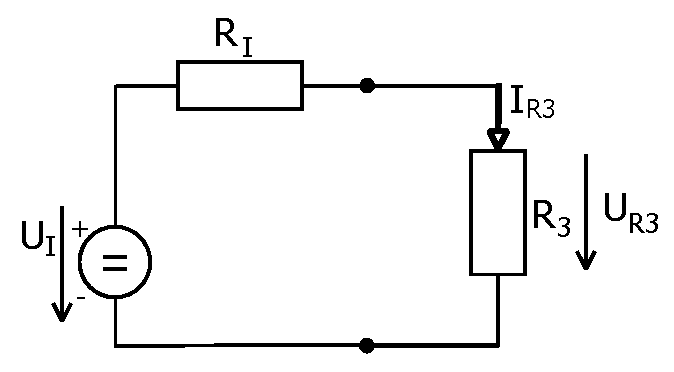
\includegraphics[width=0.6\linewidth]{obr/2_3.pdf}
		\caption{zjednodušený obvod}
	\end{figure}
Pomocí získaných hodnot si dopočítáme potřebné veličiný:	
\begin{gather*}
U_i=U_{R2}-U_{R1}=50-31.57895\doteq18.42105V\\
I_{R3}=\frac{U_i}{R_I+R_3}=\frac{18.42105}{291.22807+660}\doteq0.01937A\\
U_{R3}=R_3\cdot I_{R3}=660\cdot0.01937\doteq12.7842V
\end{gather*}